\section{Wireless Transfer}
\label{sec:wireless}
This section will cover the implementation of the data transfer. Although the decision made in the research was to use a transparent network bridge, described in section \ref{sec:tbm}, some obstacles on getting that to work well directed in switching to the listening bridge model, described in section \ref{sec:lbm}, to avoid them. The next subsections cover the set up process for the Raspberry Pi, the software written to use on the Raspberry Pi or connected systems, and why some software written was deemed unsuitable for use.
\subsection{Used existing software}
Apart from some software libraries, there are two existing software packages used to provide the required networking features. The next paragraphs will cover why hostapd and dnsmasq were selected.

Hostapd (host access point daemon) is used to set up the wireless network on the Raspberry Pi in access point mode. By providing an access point to which computers running the monitoring client can connect, bothersome networking set up is avoided. The client connects to the access point, starts the monitoring client and that is all from a networking point of view.

Unfortunately, only providing an access point is not enough to provide a smooth network set up. Most (if not all) clients that connect will try to obtain an IP-address using DHCP, and this is where dnsmasq comes in. Although the name of this package implies it provides a DNS server, this package also provides other services from which the DHCP capability is used. It is configured to assign addresses in two ranges bound to both the wireless and wired networking interface on the Raspberry PI respectively.

In contrast to the original plan, the Raspberry Pi will not create one network. Forwarding packages between the two network interfaces with iptables in the desired configuration turned out not to be possible, so the transparent bridge model was set aside and a custom forwarding solution was written. This solution will be covered in some of the following subsections.

\subsection{Scripted installation}
In order to simplify the installation of the Raspberry Pi, a set up script was written to perform the installation and configuration of the required software on the Raspberry Pi. The only requirements for running this script are a Raspberry Pi with Raspbian (the recommended Linux distribution), an internet connection and the script itself. The script will download and install all required software and configuration files.

A script written in Python accompanies the installation script to perform modifications, additions and replacement of existing configuration files and the installation of new ones in the correct locations. This part of the installation is not written in Bash to avoid the somewhat steep learning curve of doing those operations in Bash.

\subsection{Networking bridge}
Due to the switch to the listening bridge model, bridging software had to be written to run on the Raspberry Pi. The first implementation for this was a script written in Python, accompanied by a script to display some basic metrics of the system. However, after testing this implementation with the performance testing software, which will be covered later on in detail, this script was found unable to deliver the required performance. Before modifications the network was unable to process the amount of packages, and after improvements on that Python lacked performance to do the required data compression.

To leave behind all of the networking performance issues, the bridging software was rewritten in C. While staying compatible with the companion script, the system load decreased with 90\% compared with the improved script written in Python.

To cope with the performance issues as mentioned before, a solution to keep network packets under 1500 bytes (one ethernet frame on the wireless interface) was needed. When this limit is exceeded, the network layer has to break up the packets on the sender and reassemble them on the receiver, causing a severe performance hit. Our own stress test Simulink model generates packets with a size of about 7500 bytes, which can be reduced to 4500 bytes by using the deflate compression algorithm. Although this is going in the right direction, the packages are still too large by a factor of three.

The last improvement made to reach the desired packet size, was to make use of prior knowledge of the packet contents. Much of the data does not change between packets, so by using xor on the current and previous data the result will comprise many bytes with zero as value. By using deflate on this xorred data, the packet size can be reduced to less than 400 bytes. To avoid issues when packets are still lost, the first packet will be kept as reference and all the following packets will be xorred with the first.

To make sure that any connected client obtains this reference packet, a separate program was written. The bridging program will store the reference packet, and when a client sends a request for a reference packet this program will return one. Being the only program listening to requests from clients, it also handles requests for recording. This is covered a bit more in depth in the section about data recording.

\subsection{Network performance}

To gather metrics on the performance of the network setup, two programs were written to act as a replacement sender and a replacement receiver. While the basic structure of the network packets is the same as generated by the Simulink model to stay compatible with the bridging software, an unique identifier is added as payload and the remains of the packet are filled with random data. When running the software, the number of packets to be processed, the size of the packets, the number of packets per second and a log file can (and have to) be specified. Each packet will be filled with new random generated data to prevent the compression in the bridging software working too well: after all the packet size should roughly match the desired size.

With this two programs, the issues with packet loss on the wireless connection were detected. Accompanied by Wireshark they provided a way to measure the network performance and measure the effects of improvements made to the other software parts.

\begin{figure}[H]
	\centering
	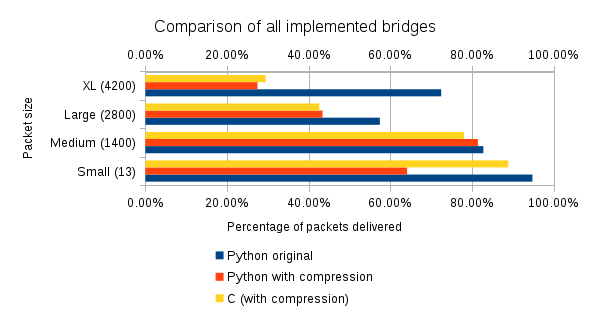
\includegraphics[width=\linewidth]{images/overview.png}
	\caption{Network performance comparison of implemented bridging variations}
	\label{fig:networkperformance}
\end{figure}

In the figure above, the networking performance of the three built implementations are compared. Although this graph might imply that the original python variant should be chosen, it would end up as a bad choise in practice. In these tests the variants with compression are forced to compress almost incompressable data, while in practice the performance is better. On top of that, a compression rate of 50\% or better is realistic. Translated to practice, this will mean that the performance in the complete input range between 13 and 2800 for the C-program will lie between range of 13 and 1400 on this graph, outperforming both implementations in Python. Another important side-note is that although the implementation in Python seems to excel when processing very large packages, it will cause a crash of the network stack on the Raspberry Pi within a minute.

\subsection{Data recorder}

A 'could have' in the requirements was the feature to record data. In the last two weeks, this functionality was added to the Raspberry Pi. The decision to add the recording feature as part of the bridging software is based on wanting to keep the impact of packet loss on the wireless connection out of the recordings. The recorder is connected to the forwwarder software with a named pipe, and writes the data without modifications to persistent storage on the Raspberry Pi.

\subsection{Retrieving data recordings}

As mentioned in the previous subsection, the stored recordings contain data as processed by the bridging software. On top of that, the recordings are stored on the Raspberry Pi. To retrieve this recordings, and to convert the data to a readable format (for Matlab, Excel or other tool for data processing), a couple of programs were written. The convert program will convert a given recording to a tab-separated file, and the web server will list all the recordings. The later will call the convert program to send a converted recording to a client.